\begin{figure}
\begin{center}
\begin{tikzpicture}[>=latex,thick]
%\draw (-7,-15.8) rectangle (7,2.7);
\clip (-7,-15.8) rectangle (7,2.7);
\begin{scope}
\node at (0,0) {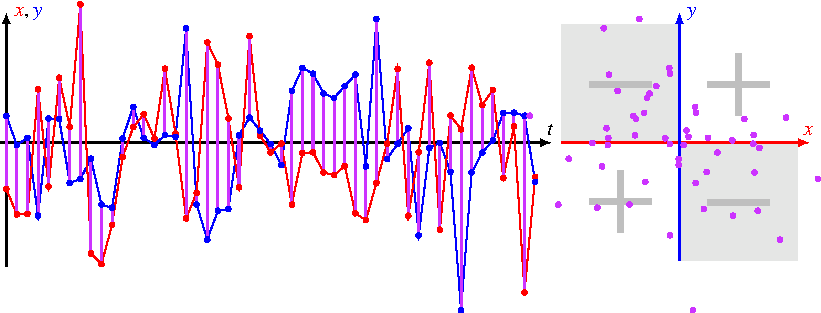
\includegraphics{chapters/000-einleitung/images/randrand.pdf}};
\end{scope}
\begin{scope}[yshift=-4.5cm]
\node at (0,0) {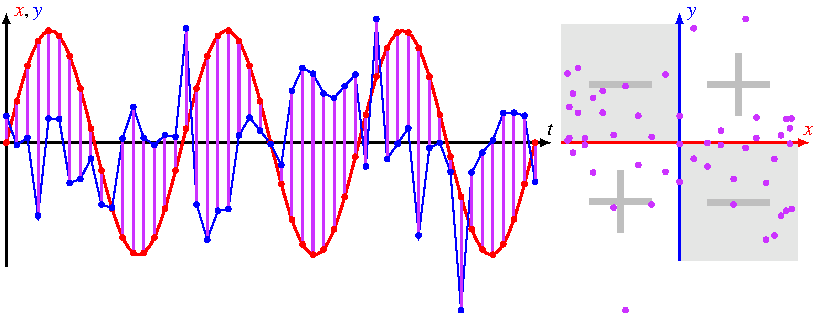
\includegraphics{chapters/000-einleitung/images/sinrand.pdf}};
\end{scope}
\begin{scope}[yshift=-9.0cm]
\node at (0,0) {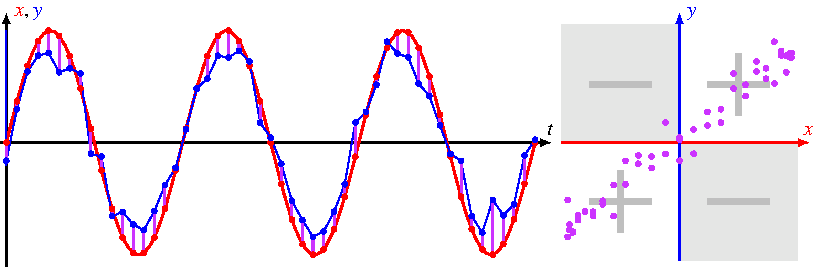
\includegraphics{chapters/000-einleitung/images/sinsin.pdf}};
\end{scope}
\begin{scope}[yshift=-13.5cm]
\node at (0,0) {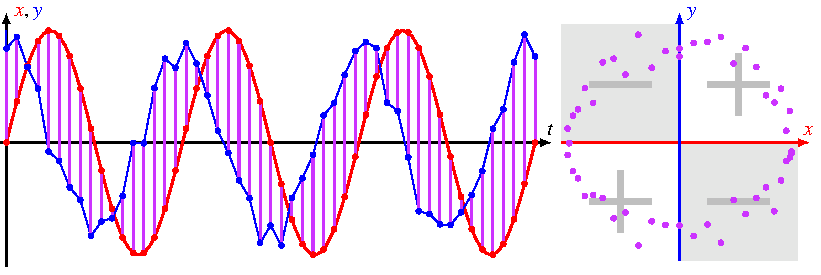
\includegraphics{chapters/000-einleitung/images/sincos.pdf}};
\end{scope}
\end{tikzpicture}
\end{center}
\caption{Stichproben verschiedener Zufallsvariablen mit unterschiedlich
ausgeprägter Kovarianz
\label{buch:einleitung:fig:kovvergleich}}
\end{figure}
